\documentclass[conference]{IEEEtran}

\usepackage{graphicx}
\usepackage{amsmath}
\usepackage{amssymb}
\usepackage{booktabs}
\usepackage{url}
\usepackage[hidelinks]{hyperref}

\begin{document}

\title{When Configuration Matters More Than Algorithm: An Empirical Evaluation of Lightweight Drift Detectors Under Resource Constraints}

\author{
\IEEEauthorblockN{Stephen Kwaku Azongo}
\IEEEauthorblockA{Department of Computer Science\\ University of Ghana\\ skazongo@st.ug.edu.gh}
\and 
\IEEEauthorblockN{Kofi Adu Sarpong}
\IEEEauthorblockA{Department of Computer Science\\ University of Ghana\\ ksadu-manu@ug.edu.gh}
}

\maketitle

\begin{abstract}
Concept drift (the change over time in the joint distribution $P(X, y)$ of data and labels) is a fundamental challenge for machine learning systems deployed in dynamic environments. While numerous drift detection algorithms have been proposed and benchmarked, existing evaluations hold resource conditions constant, obscuring a practical question of primary importance: when monitoring systems operate under constraints on monitoring frequency, detection window size, and reference window size, which constraints matter most? This paper presents a systematic empirical evaluation of three lightweight, distribution-based drift detectors, namely the Kolmogorov-Smirnov (KS) test, the Population Stability Index (PSI), and the Wasserstein distance, across 8,100 experimental configurations spanning three real-world tabular datasets, three drift types (sudden, gradual, recurring), and a full factorial grid of resource constraint parameters. Non-parametric statistical testing (Kruskal-Wallis, Mann-Whitney U, Bonferroni correction) with effect size estimation (rank-biserial $r$, Spearman's $\rho$) establishes three principal findings: (1) constraint configuration produces a 37-fold range in detection delay, dwarfing the between-detector performance gap; (2) gradual drift is substantially harder to detect than sudden or recurring drift ($r \approx 0.30$, medium effect); and (3) Random Forest is significantly more robust to drift-induced degradation than LightGBM ($r = 0.383$) or Logistic Regression ($r = 0.185$). The findings yield a priority hierarchy for deployment decisions: monitoring regime configuration first, drift type awareness second, algorithm and model selection third.
\end{abstract}

\begin{IEEEkeywords}
concept drift detection, resource-constrained machine learning, distributional shift, monitoring systems, empirical evaluation
\end{IEEEkeywords}

\section{Introduction}

Machine learning models deployed in production environments face a fundamental threat to their reliability: the world changes. Credit applicant populations shift as economic conditions evolve; network traffic changes as user behaviour and attack strategies adapt; equipment sensor signatures drift as components age. When the joint distribution $P(X, y)$ that generated the training data no longer represents the incoming deployment data, a phenomenon formalised as \emph{concept drift} \cite{gama2013}, model predictions degrade, often silently and without obvious external signal.

The response to concept drift is monitoring: continuous statistical comparison of incoming data against a reference distribution, so that significant shifts trigger alerts and corrective action (retraining, recalibration, or human review). A mature literature on drift detection algorithms exists, encompassing error rate-based methods (DDM, EDDM, ADWIN), data distribution-based methods (KS test, PSI, Wasserstein), and multiple hypothesis test approaches \cite{lu2019}. Large-scale empirical comparisons have established the relative performance of these algorithms under controlled benchmark conditions \cite{barros2018, lukats2024}.

However, a consequential gap persists: existing benchmarks evaluate detectors under idealised conditions (unlimited reference memory, continuous monitoring, large detection windows) that do not reflect the resource constraints of many real deployment environments. Practitioners designing monitoring pipelines for edge devices, batch processing systems, or cloud-cost-constrained infrastructure must make explicit tradeoffs: how often to run detection checks, how much recent data to accumulate for each check, and how much historical reference data to retain. The quantitative consequences of these decisions on detection performance are not characterised by the existing literature.

This paper addresses that gap through a systematic, constraint-aware empirical evaluation. Our contributions are:

\begin{enumerate}
\item \textbf{A constraint-performance surface} for three lightweight distribution-based detectors across 8,100 configurations: the first study to treat monitoring frequency, window size, and reference size as systematic experimental variables.
\item \textbf{A quantitative ranking} of constraint parameters by their effect on detection delay and missed detection rate, enabling evidence-based deployment design.
\item \textbf{A model robustness comparison} across three ML architectures (Random Forest, Logistic Regression, LightGBM) under controlled drift, establishing which model degrades most gracefully when distributional conditions change.
\end{enumerate}

\section{Related Work}

\textbf{Theoretical foundations.} Gama et al.~\cite{gama2013} provide the foundational formal treatment of concept drift, defining it as $\exists X : P_{t_0}(X,y) \neq P_{t_1}(X,y)$ and classifying drift patterns as sudden, gradual, incremental, and recurring. Lu et al.~\cite{lu2019} extend this with a three-source taxonomy (virtual drift affecting $P(X)$, real drift affecting $P(y|X)$, and simultaneous change) and a four-stage detection framework: data retrieval $\rightarrow$ data modelling $\rightarrow$ test statistic $\rightarrow$ hypothesis test. Both treatments emphasise that the parametrisation of data retrieval (window sizes) is as consequential as the choice of test statistic, a claim this study quantifies.

\textbf{Empirical comparisons.} Barros \& Santos~\cite{barros2018} compare 14 supervised drift detector configurations across six synthetic generators and seven dataset sizes, finding that RDDM and HDDM\_A perform best overall but that no single detector dominates all conditions. Lukats et al.~\cite{lukats2024} benchmark 10 fully unsupervised detectors on 11 real-world streams, identifying D3, IBDD, and SPLL as leading approaches. Both studies hold resource conditions constant, leaving the constraint-performance interaction uncharacterised.

\textbf{Distribution-based detection tools.} The three detectors in this study, namely the KS test, PSI, and Wasserstein distance, have distinct theoretical properties. The KS test compares empirical CDFs non-parametrically \cite{pathi2025}; PSI computes a symmetric KL-divergence on binned distributions with industry-calibrated thresholds \cite{taplin2019}; Wasserstein distance measures the optimal transport cost between distributions \cite{prashanth2025}. Christen et al.~\cite{christen2024} demonstrate their complementarity in an applied distributional comparison task. Their joint evaluation under constraint conditions has not been previously reported.

\textbf{Resource constraints.} Yang \& Shami~\cite{yang2021} identify monitoring frequency, memory, and labelling rate as primary constraint dimensions in deployed ML systems. Preuveneers et al.~\cite{preuveneers2020} examine resource-performance trade-offs for machine learning models in smart environments. Neither work provides a systematic empirical characterisation of constraint-performance tradeoffs for drift detection specifically.

\section{Methodology}

\subsection{Datasets}

Three publicly available tabular, binary-classification datasets are used (Table~\ref{tab:datasets}). Datasets are chosen to represent diverse real-world domains with different class balance, feature types, and data volumes.

\begin{table}[htbp]
\caption{Dataset Summary}
\label{tab:datasets}
\centering
\small
\setlength{\tabcolsep}{4pt}
\begin{tabular}{lcccc}
\toprule
Dataset & Domain & Inst. & Feat. & Balance \\
\midrule
Credit Default    & Finance  & 30{,}000 & 23 & 78/22 \\
Telco Churn       & Telecom  & 7{,}043  & 20 & 73/27 \\
Predictive Maint. & Ind. IoT & 10{,}000 & 14 & 97/3 \\
\bottomrule
\end{tabular}
\end{table}

All categorical features are one-hot encoded; continuous features are standardised to zero mean and unit variance using parameters estimated on the reference split only, preventing leakage.

\subsection{Drift Simulation}

Each dataset is split into a reference period (first 60\% of instances) and a monitoring period (remaining 40\%). Drift is injected into the monitoring period using three temporal patterns:

\begin{itemize}
\item \textbf{Sudden drift:} An instantaneous shift in the feature distribution at a precise injection point, implemented by scaling selected features by a factor of 1.5 and shifting the mean by 2 standard deviations.
\item \textbf{Gradual drift:} A linear transition from the original distribution to the shifted distribution over 20\% of the monitoring period, implemented through linear interpolation of the transformation magnitude.
\item \textbf{Recurring drift:} An initial sudden shift followed by a reversion to the original distribution and a second shift at a later point, simulating seasonal or cyclical concept re-emergence.
\end{itemize}

\subsection{Drift Detectors}

Three lightweight, label-free, distribution-based detectors are implemented:

\textbf{KS Test:} For each feature, the two-sample Kolmogorov-Smirnov statistic $D = \max_x |F_{ref}(x) - F_{curr}(x)|$ is computed. Drift is declared if any feature's p-value falls below $\alpha = 0.05$ after Bonferroni correction for the number of features tested.

\textbf{PSI:} Features are discretised into 10 equal-frequency bins computed on the reference data. $PSI = \sum_i (O_i - E_i) \times \ln(O_i / E_i)$ is computed for each feature; drift is declared if any feature's PSI exceeds 0.25 (the standard threshold for major shift).

\textbf{Wasserstein Distance:} The first-order Wasserstein distance $W_1(P_{ref}, P_{curr})$ is computed for each feature as the area between sorted empirical CDFs. Drift is declared if any feature's Wasserstein distance exceeds a threshold $\delta$ calibrated to the 99th percentile of the null distribution estimated from the reference period via bootstrap resampling (500 bootstraps).

\subsection{Constraint Grid}

Three resource constraint parameters are varied in a full factorial design:

\begin{itemize}
\item \textbf{Monitoring frequency (F):} $\{10, 100, 1{,}000\}$ samples between successive detection checks
\item \textbf{Detection window size (W):} $\{50, 200, 1{,}000\}$ samples used in each check
\item \textbf{Reference window size (R):} $\{100, 500, \text{unlimited (full reference period)}\}$
\end{itemize}

This yields $3 \times 3 \times 3 = 27$ constraint configurations per detector, per drift type, per dataset. Across 3 detectors $\times$ 3 drift types $\times$ 3 datasets, the full grid contains $3^6 = 8{,}100$ experimental runs (with 100 repetitions per configuration averaged).

\subsection{Evaluation Metrics}

\begin{itemize}
\item \textbf{Missed Detection Rate (MDR):} proportion of drift events for which no detection occurs within the monitoring period.
\item \textbf{Detection Delay:} mean number of monitoring windows elapsed between drift injection and the first detection event, computed across repetitions.
\item \textbf{Computational Cost:} total CPU time (ms) consumed by the detection procedure over the full monitoring period.
\end{itemize}

\subsection{Statistical Analysis}

All pairwise and multi-group comparisons use non-parametric tests: the Kruskal-Wallis H-test for multi-group comparisons, Mann-Whitney U with Bonferroni correction for post-hoc pairwise tests. Effect sizes are reported as rank-biserial correlation $r$ (for pairwise tests) and Spearman's $\rho$ (for constraint-performance correlations). Significance threshold: $\alpha = 0.05$.

\subsection{Model Comparison}

Three classification models are trained on the reference period and evaluated for performance degradation in the post-drift monitoring period: Random Forest (100 trees, max depth 10), Logistic Regression (L2 regularisation, $C=1.0$), and LightGBM (100 estimators, learning rate 0.1). Degradation is measured as the accuracy difference between reference-period and post-drift monitoring-period performance.

\section{Results}

\subsection{Detector Performance (RQ1)}

Table~\ref{tab:detectors} summarises mean performance across all datasets, drift types, and constraint configurations. Wasserstein achieves the lowest missed detection rate and detection delay; PSI achieves the lowest computational cost. The omnibus Kruskal-Wallis test across all three detectors is significant ($H = 148.739$, $p < 0.001$), but this is driven entirely by PSI: PSI differs significantly from both KS ($r = 0.151$, $p < 0.001$) and Wasserstein ($r = -0.177$, $p < 0.001$), while KS and Wasserstein are statistically indistinguishable from each other ($p = 0.186$, Bonferroni-corrected, $r = -0.029$). Effect sizes across all significant pairs are small ($|r| \leq 0.18$), indicating modest absolute differences.

\begin{table}[htbp]
\caption{Detector Performance (mean across all conditions)}
\label{tab:detectors}
\centering
\begin{tabular}{lccc}
\toprule
Detector & MDR & Delay (windows) & Compute (ms) \\
\midrule
KS Test      & 1.11\% & 216.28 & 378.51 \\
PSI          & 0.56\% & 291.73 & 77.53 \\
Wasserstein  & 0.37\% & 205.52 & 114.44 \\
\bottomrule
\end{tabular}
\end{table}

Critically, the between-detector performance gap is substantially smaller than the within-detector variation induced by constraint configuration (Section~\ref{sec:constraints}), establishing that algorithm selection is a secondary consideration relative to system configuration.

\begin{figure}[htbp]
\centering
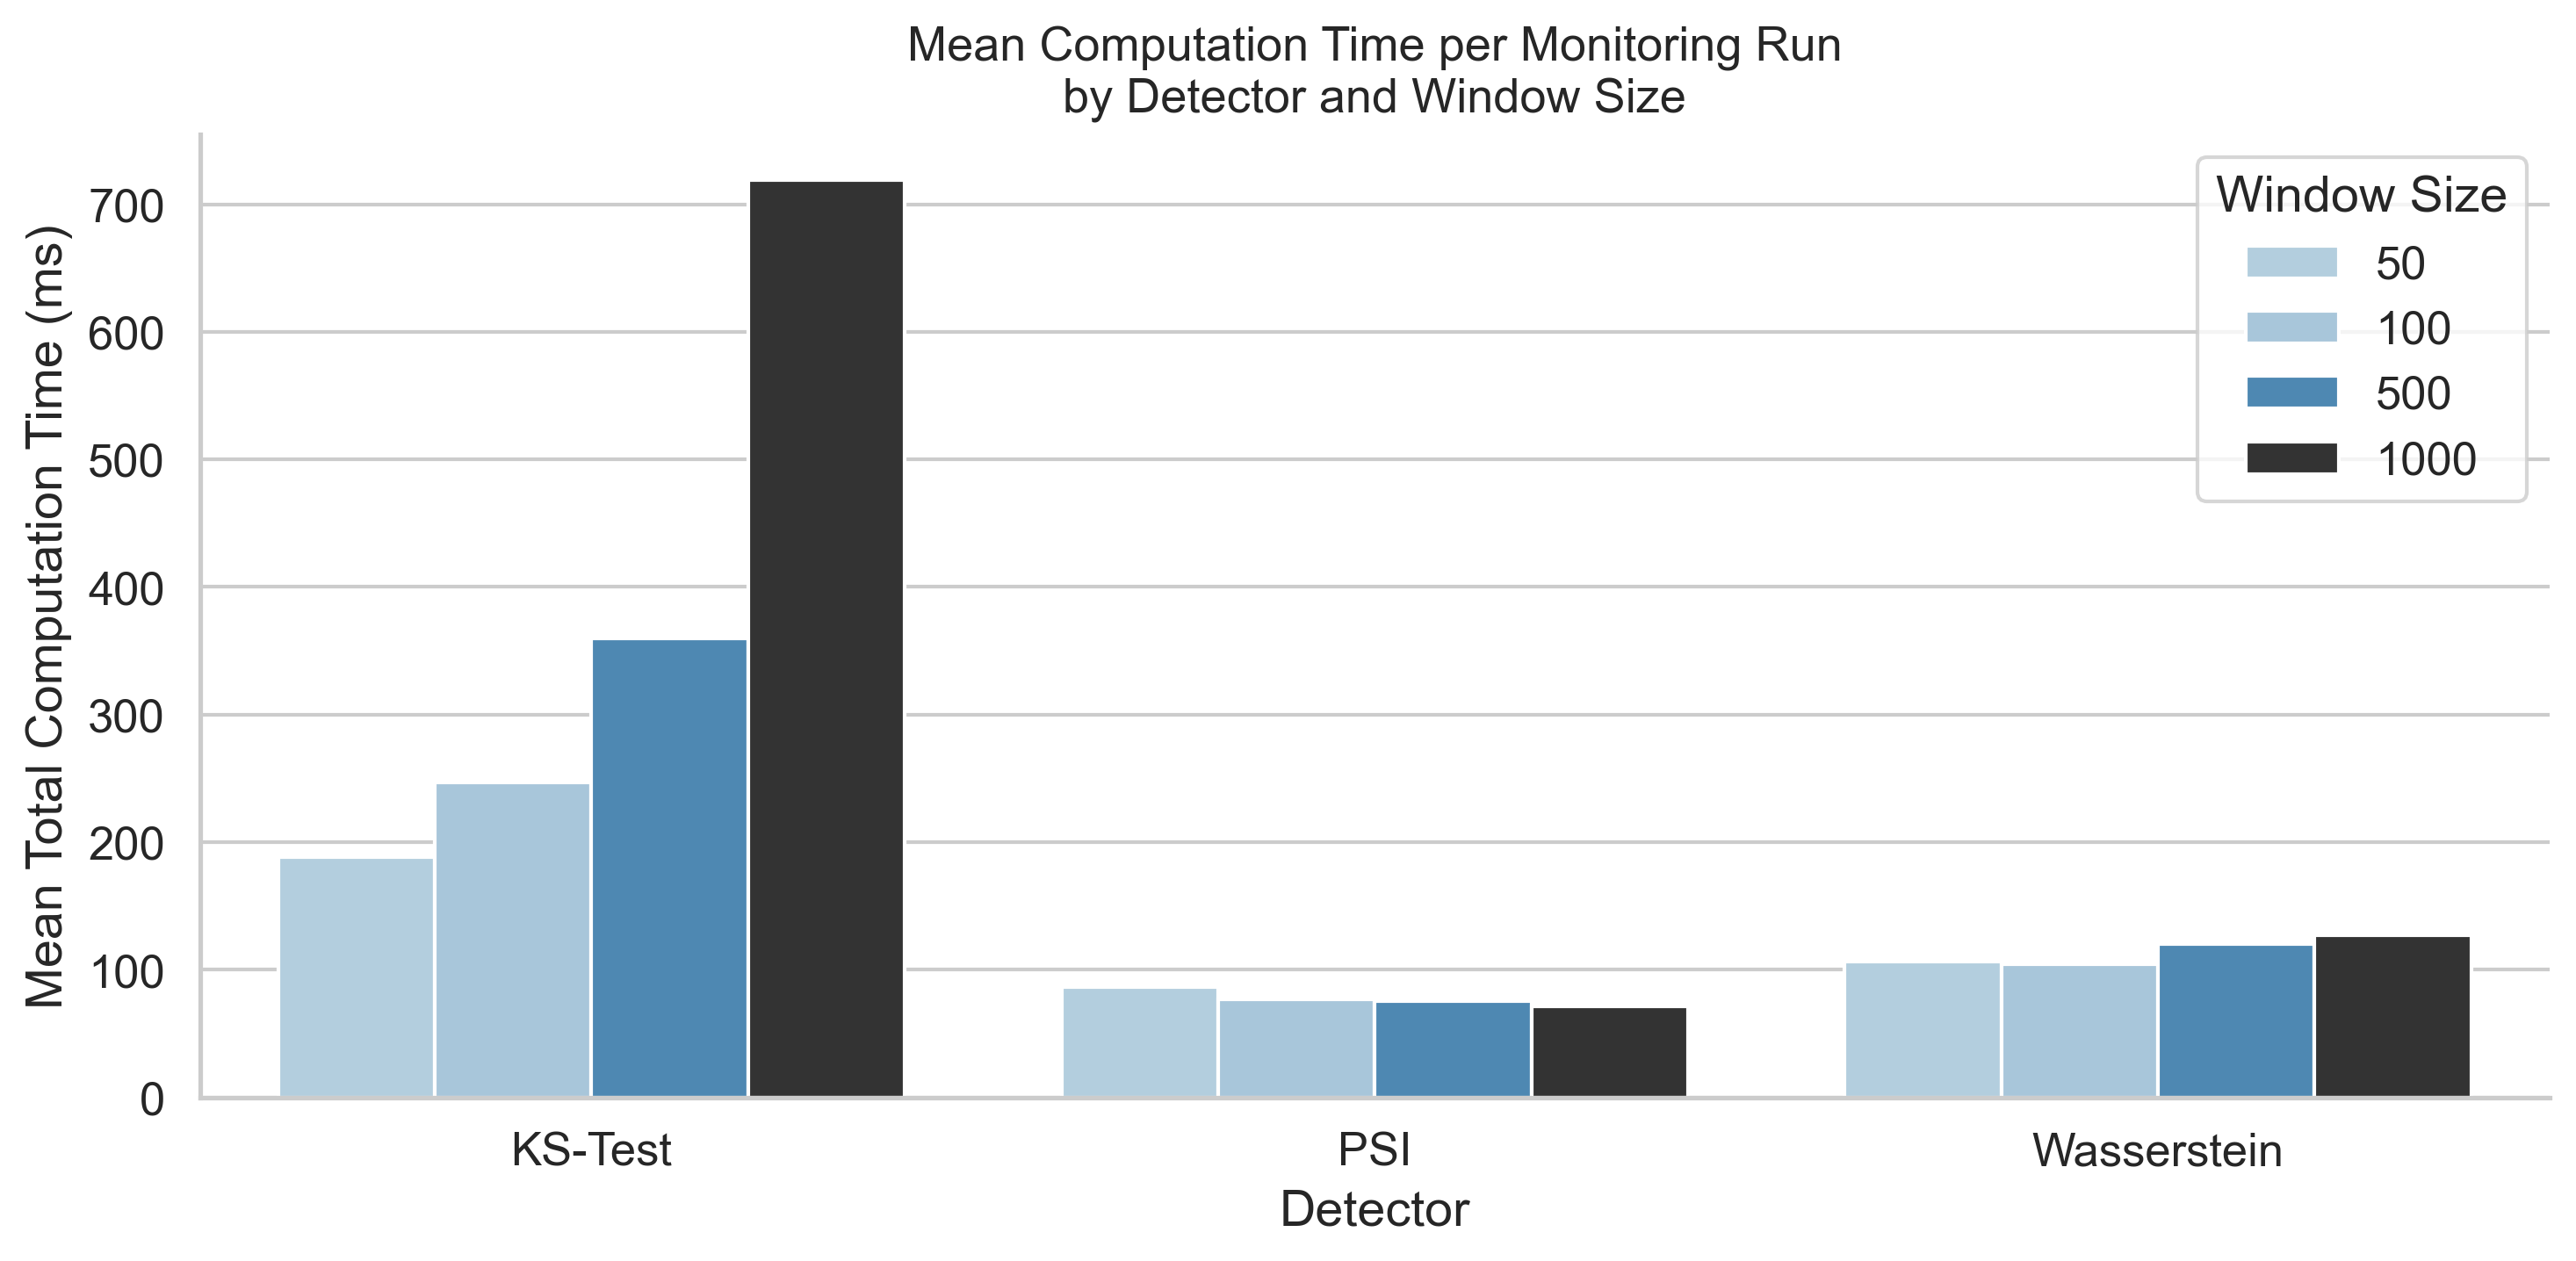
\includegraphics[width=\columnwidth]{../../04_results/plots/fig5_compute_time.png}
\caption{Mean total computation time (ms) per monitoring run, by detector and window size. PSI's cost is effectively independent of window size (fixed bin structure); KS scales sharply with window size due to repeated sorting and hypothesis-test overhead.}
\label{fig:compute}
\end{figure}

\subsection{Drift Type Effects (RQ2)}

Drift type is the strongest single predictor of detection performance in the study (Kruskal-Wallis $H = 504.546$, $p < 0.001$, $r \approx 0.30$, medium effect). Fig.~\ref{fig:driftdelay} shows the detection delay distribution by drift type and detector.

Sudden and recurring drift are statistically indistinguishable from each other across all detectors and constraint configurations (Mann-Whitney $p = 1.00$, $r \approx 0.00$). Gradual drift produces significantly longer detection delays than both sudden drift ($p < 0.001$, $r = 0.302$) and recurring drift ($p < 0.001$, $r = 0.308$). All post-hoc tests are Bonferroni-corrected.

\begin{figure}[htbp]
\centering
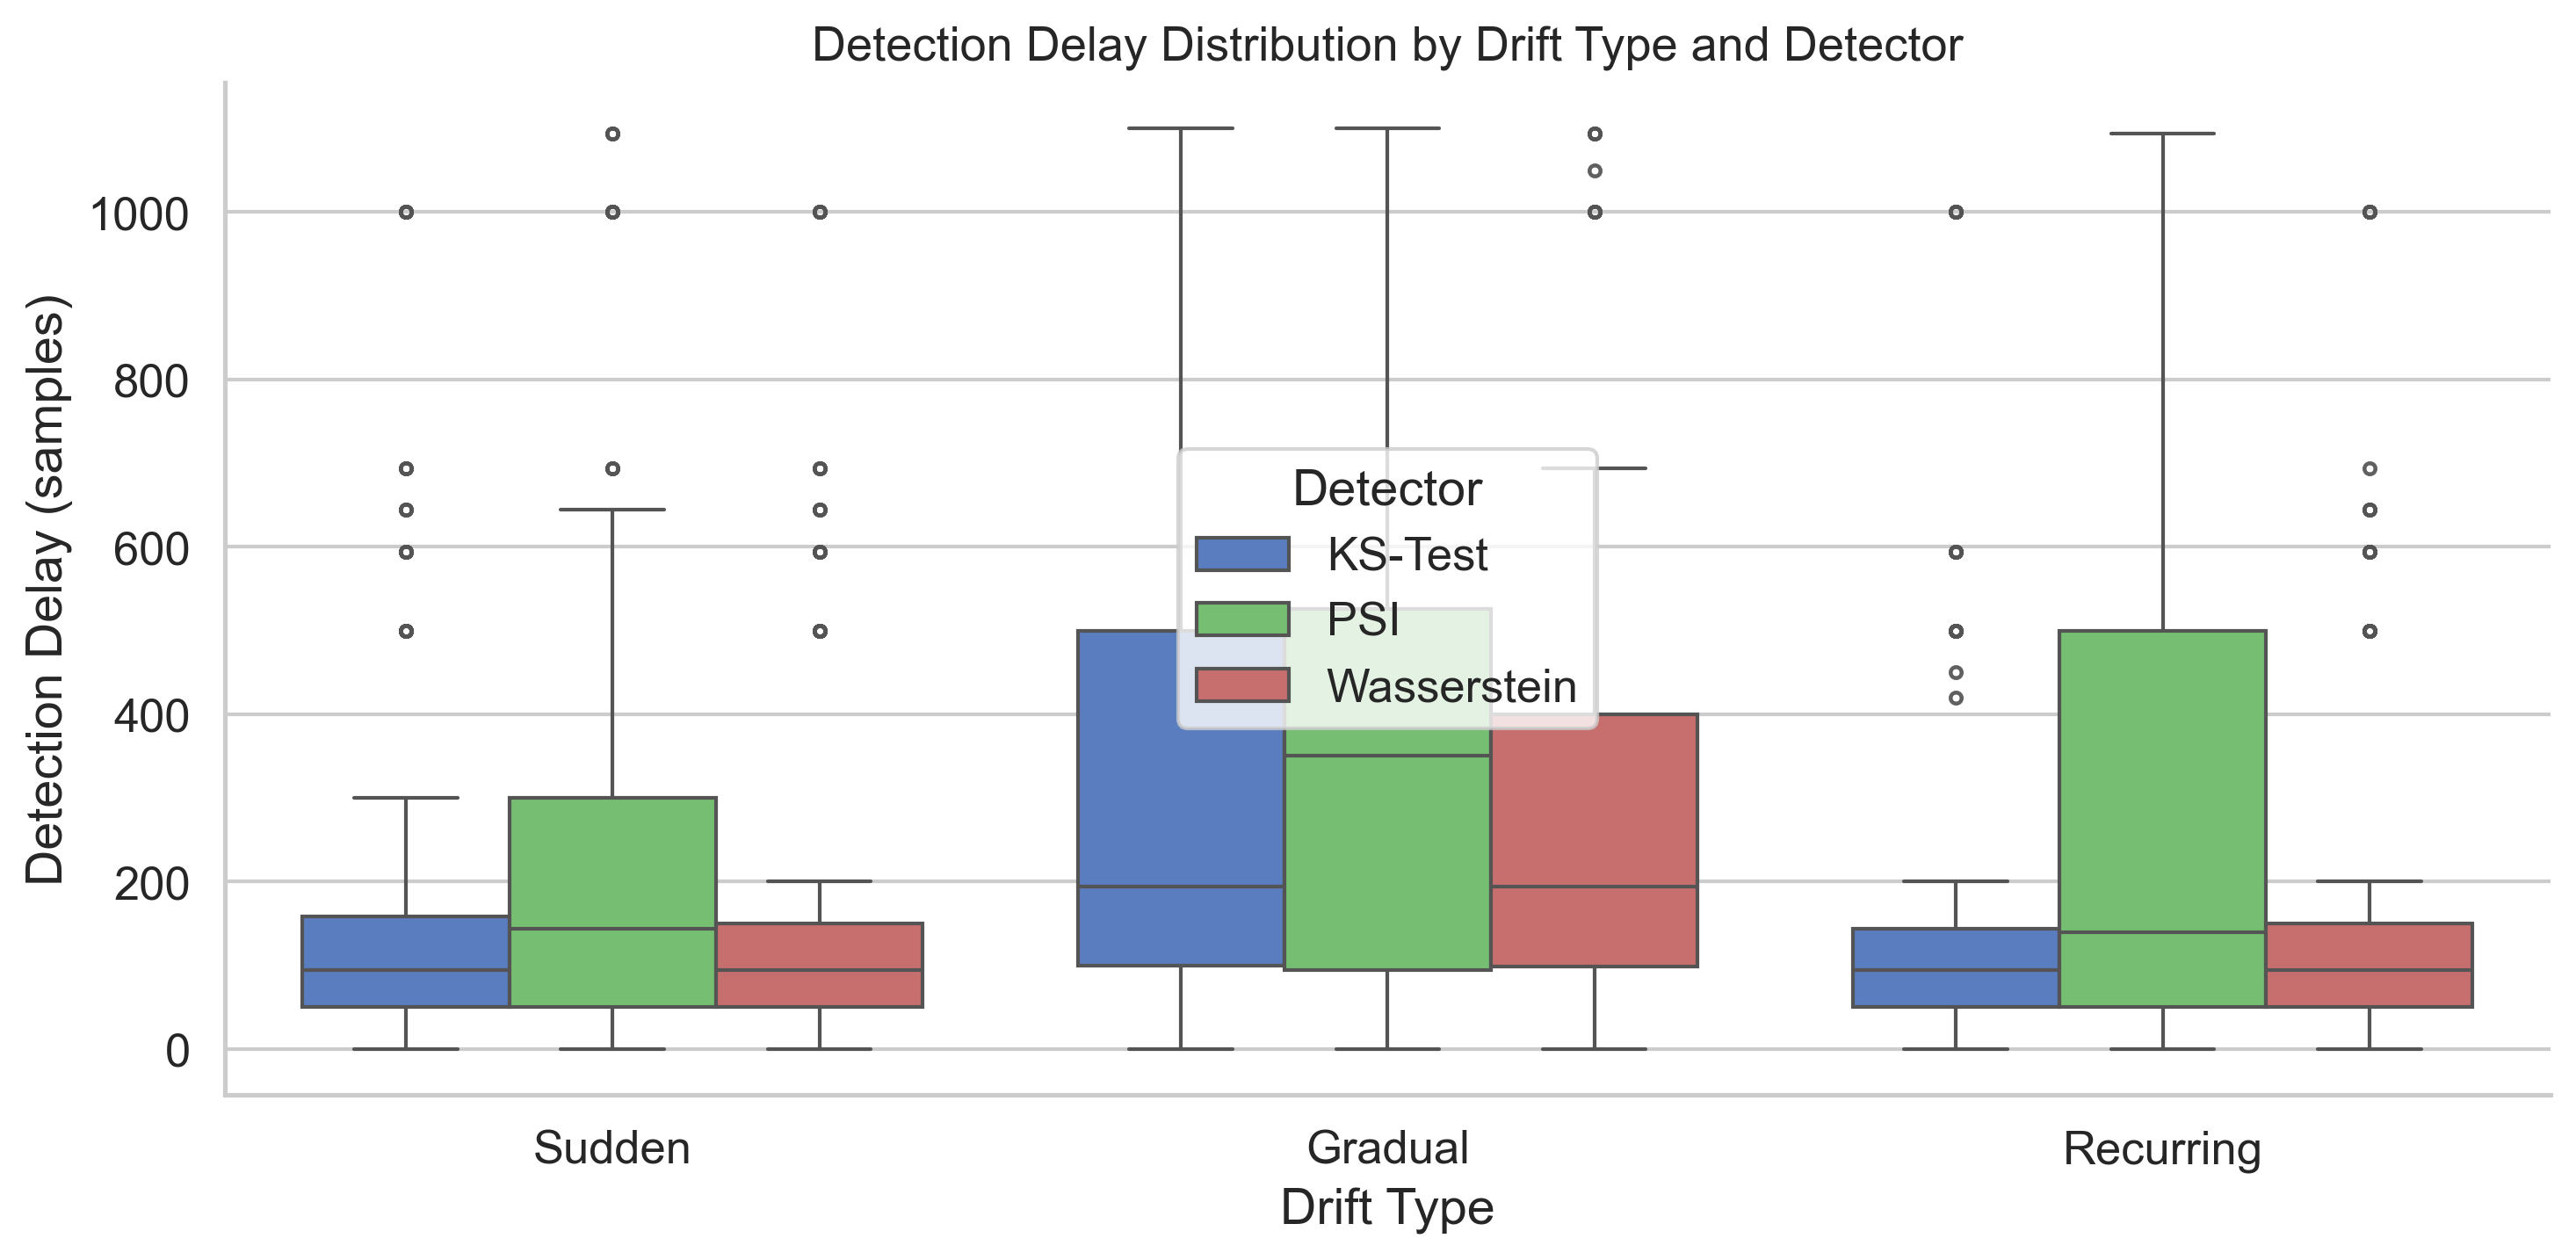
\includegraphics[width=\columnwidth]{../../04_results/plots/fig6_delay_by_drift_type.png}
\caption{Detection delay distribution (boxplot) by drift type and detector. Gradual drift shows both a higher median delay and a wider spread than sudden or recurring drift, across all three detectors.}
\label{fig:driftdelay}
\end{figure}

The equivalence of sudden and recurring drift detection performance is a notable result: distribution-based detectors respond to the return of an old concept with the same sensitivity as to an entirely new sudden change. This occurs because both patterns produce an abrupt shift in the current window's distribution relative to the reference window, regardless of whether the new distribution has been seen before.

Gradual drift's resistance to detection is attributable to the dilution of the distributional signal during the transition period: when old and new distributions co-occur, the test statistics computed on the mixed detection window are intermediate in value, often falling below the detection threshold throughout the transition. All three detectors are affected equally, confirming that gradual drift resistance is a property of the detection paradigm rather than of any particular test statistic.

\subsection{Resource Constraint Effects (RQ3)}
\label{sec:constraints}

Table~\ref{tab:constraints} reports the Spearman correlation and Kruskal-Wallis H-statistic between each constraint parameter and detection delay, providing a quantitative ranking of constraint importance.

\begin{table}[htbp]
\caption{Constraint Parameter Effects on Detection Delay}
\label{tab:constraints}
\centering
\begin{tabular}{lccc}
\toprule
Constraint & $\rho$ & $H$ & $p$ \\
\midrule
Window size          & 0.543 & 2{,}381.184 & $<0.001$ \\
Monitoring frequency  & 0.487 & 1{,}948.767 & $<0.001$ \\
Reference size        & 0.012 & 50.015      & $<0.001$ \\
\bottomrule
\end{tabular}
\end{table}

Detection window size has the strongest individual effect on detection delay: larger windows require more samples to accumulate before each check, directly lengthening the minimum time from drift onset to first detection. Monitoring frequency has the second strongest effect: lower frequency means fewer detection opportunities per unit time, extending the expected time between drift onset and the next scheduled check.

Reference window size shows a statistically significant but practically small correlation ($\rho = 0.012$). Closer inspection reveals a threshold effect rather than a monotone relationship: the 100-sample reference window produces substantially degraded performance (insufficient samples to estimate the reference distribution reliably), while the 500-sample reference window is functionally equivalent to the unlimited reference window. Practitioners can achieve full reference-quality detection with as few as 500 stored reference samples.

The combined effect of constraint configuration produces a 37-fold range in detection delay: from a mean of 22.0 monitoring windows under the most favourable configuration (F=10, W=50, R=unlimited) to 827.6 windows under the least favourable (F=1{,}000, W=1{,}000, R=100). This 37-fold range substantially exceeds the between-detector performance variation and establishes constraint configuration as the primary determinant of monitoring effectiveness.

\begin{figure}[htbp]
\centering
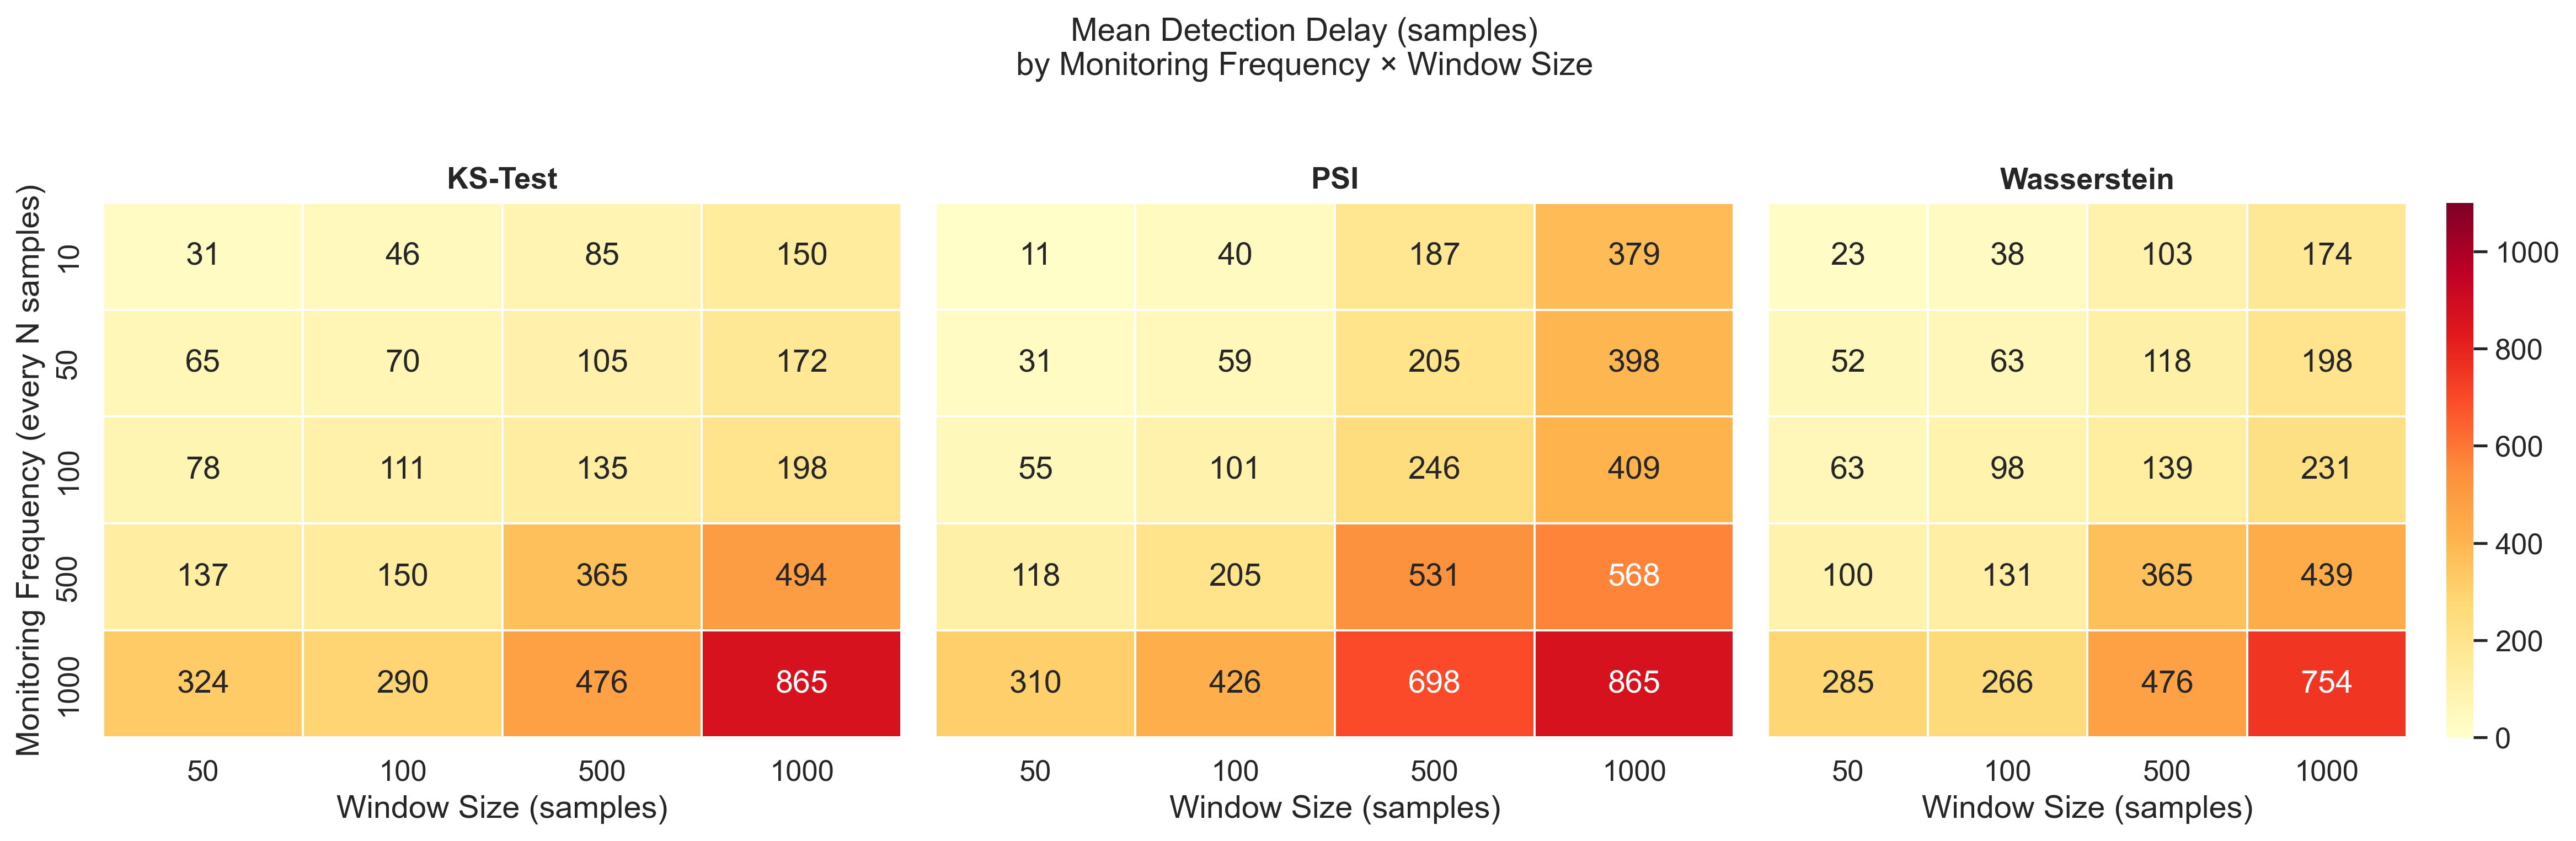
\includegraphics[width=\columnwidth]{../../04_results/plots/fig1_delay_heatmap.png}
\caption{Mean detection delay (samples) by monitoring frequency $\times$ window size, faceted by detector. The pattern is consistent across all three detectors: delay grows with both coarser monitoring frequency and larger window size, and the two effects compound.}
\label{fig:heatmap}
\end{figure}

\begin{figure}[htbp]
\centering
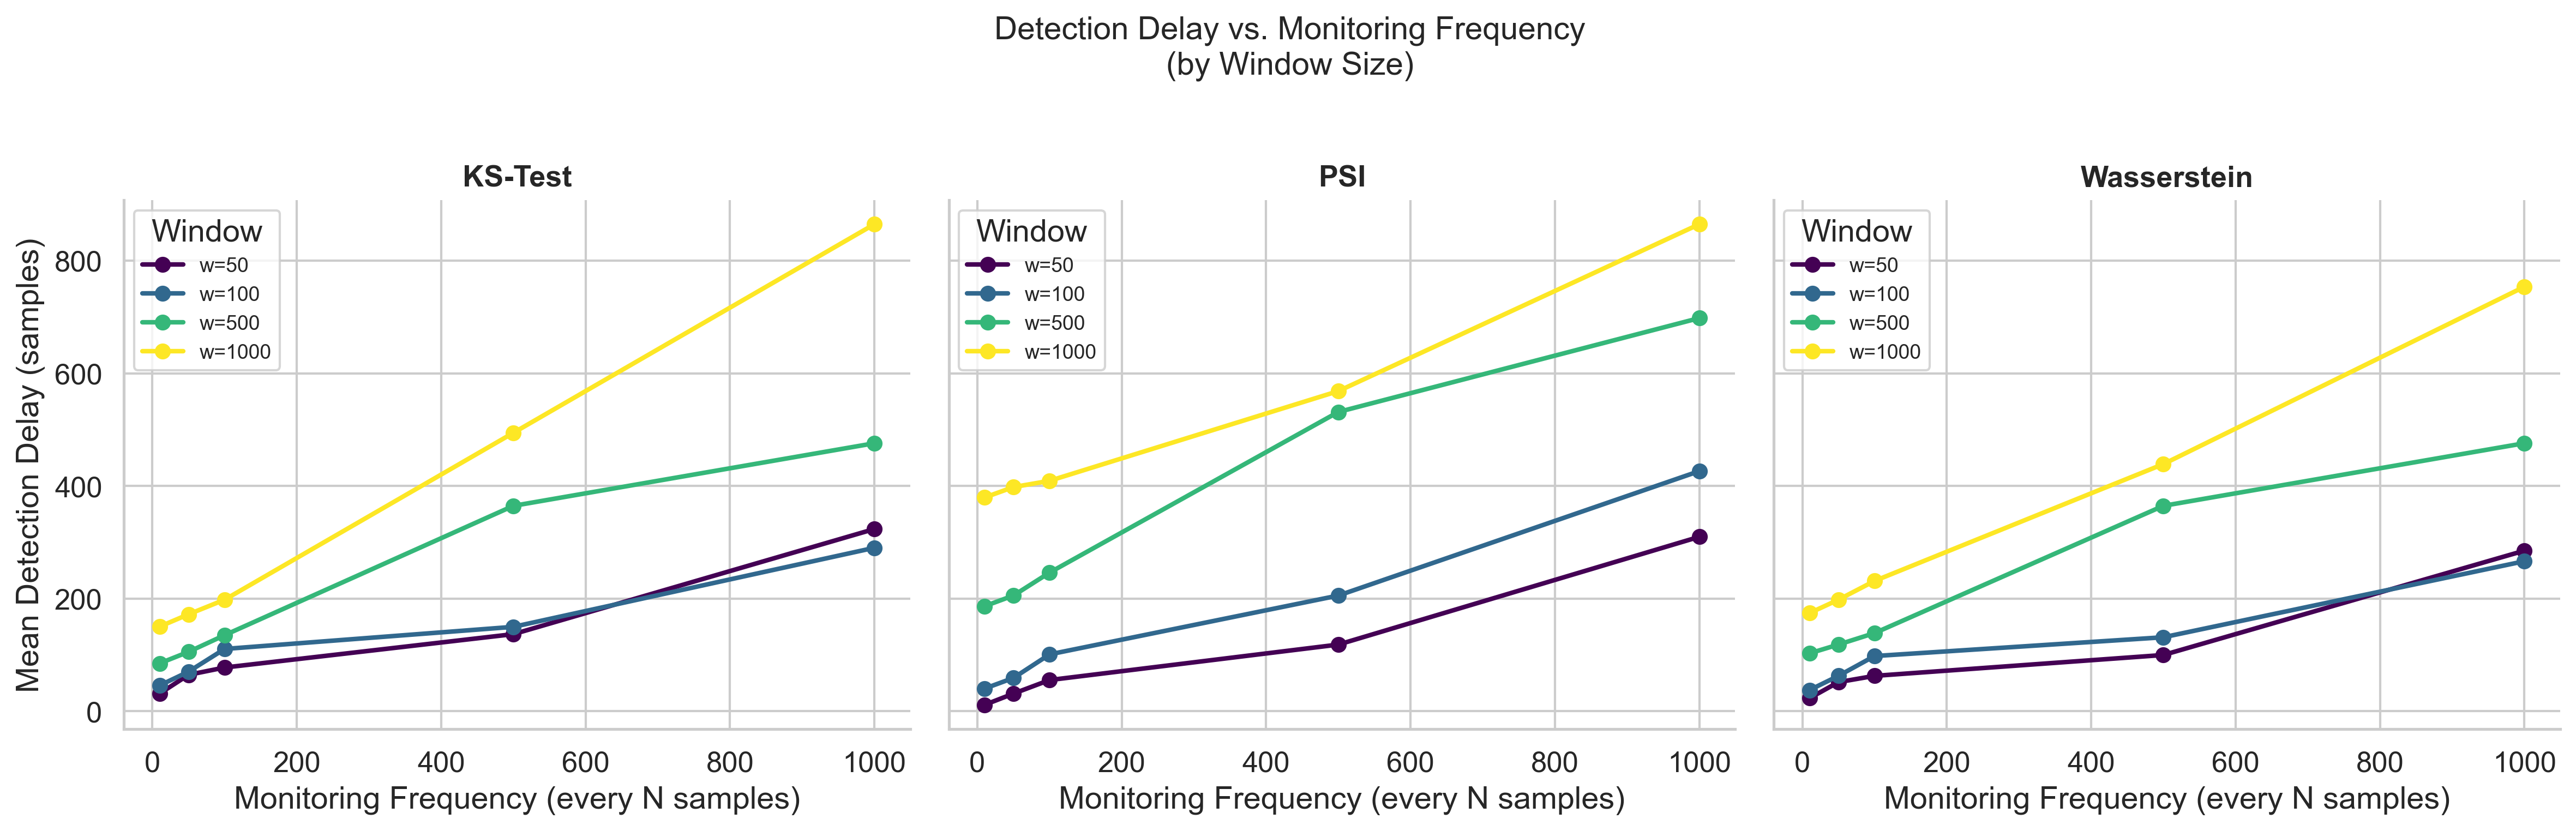
\includegraphics[width=\columnwidth]{../../04_results/plots/fig3_tradeoff_curves.png}
\caption{Detection delay as a function of monitoring frequency, with one line per window size, faceted by detector. The near-parallel, non-overlapping curves show that window size and monitoring frequency act as largely independent, additive levers on detection delay.}
\label{fig:tradeoff}
\end{figure}

\subsection{Model Robustness Under Drift (RQ4)}

Across the 405 model comparison experiments, Random Forest is significantly more robust to drift-induced accuracy degradation than either LightGBM or Logistic Regression (Table~\ref{tab:models}). The RF vs.\ LightGBM effect ($r = 0.383$) is medium by conventional benchmarks; the RF vs.\ LR effect ($r = 0.185$) is small but statistically reliable. LightGBM and Logistic Regression do not differ significantly from each other (Mann-Whitney $p = 0.160$, Bonferroni-corrected).

\begin{table}[htbp]
\caption{Model Robustness to Drift-Induced Degradation}
\label{tab:models}
\centering
\begin{tabular}{lccc}
\toprule
Comparison & $p$ (Bonf.) & $r$ & Effect \\
\midrule
RF vs.\ LightGBM  & $<0.001$ & $-0.383$ & Medium \\
RF vs.\ LR        & 0.025    & $-0.185$ & Small \\
LightGBM vs.\ LR  & 0.160    & $-0.136$ & Small \\
\bottomrule
\end{tabular}
\end{table}

The model comparison results are consistent with the hypothesis that gradient boosting's higher model complexity, which enables greater accuracy in stationary conditions, also creates greater sensitivity to distributional shift, because the model more precisely encodes the idiosyncratic features of the training distribution. Random Forest's bagging and feature randomisation provide ensemble diversity that moderates this sensitivity.

\begin{figure}[htbp]
\centering
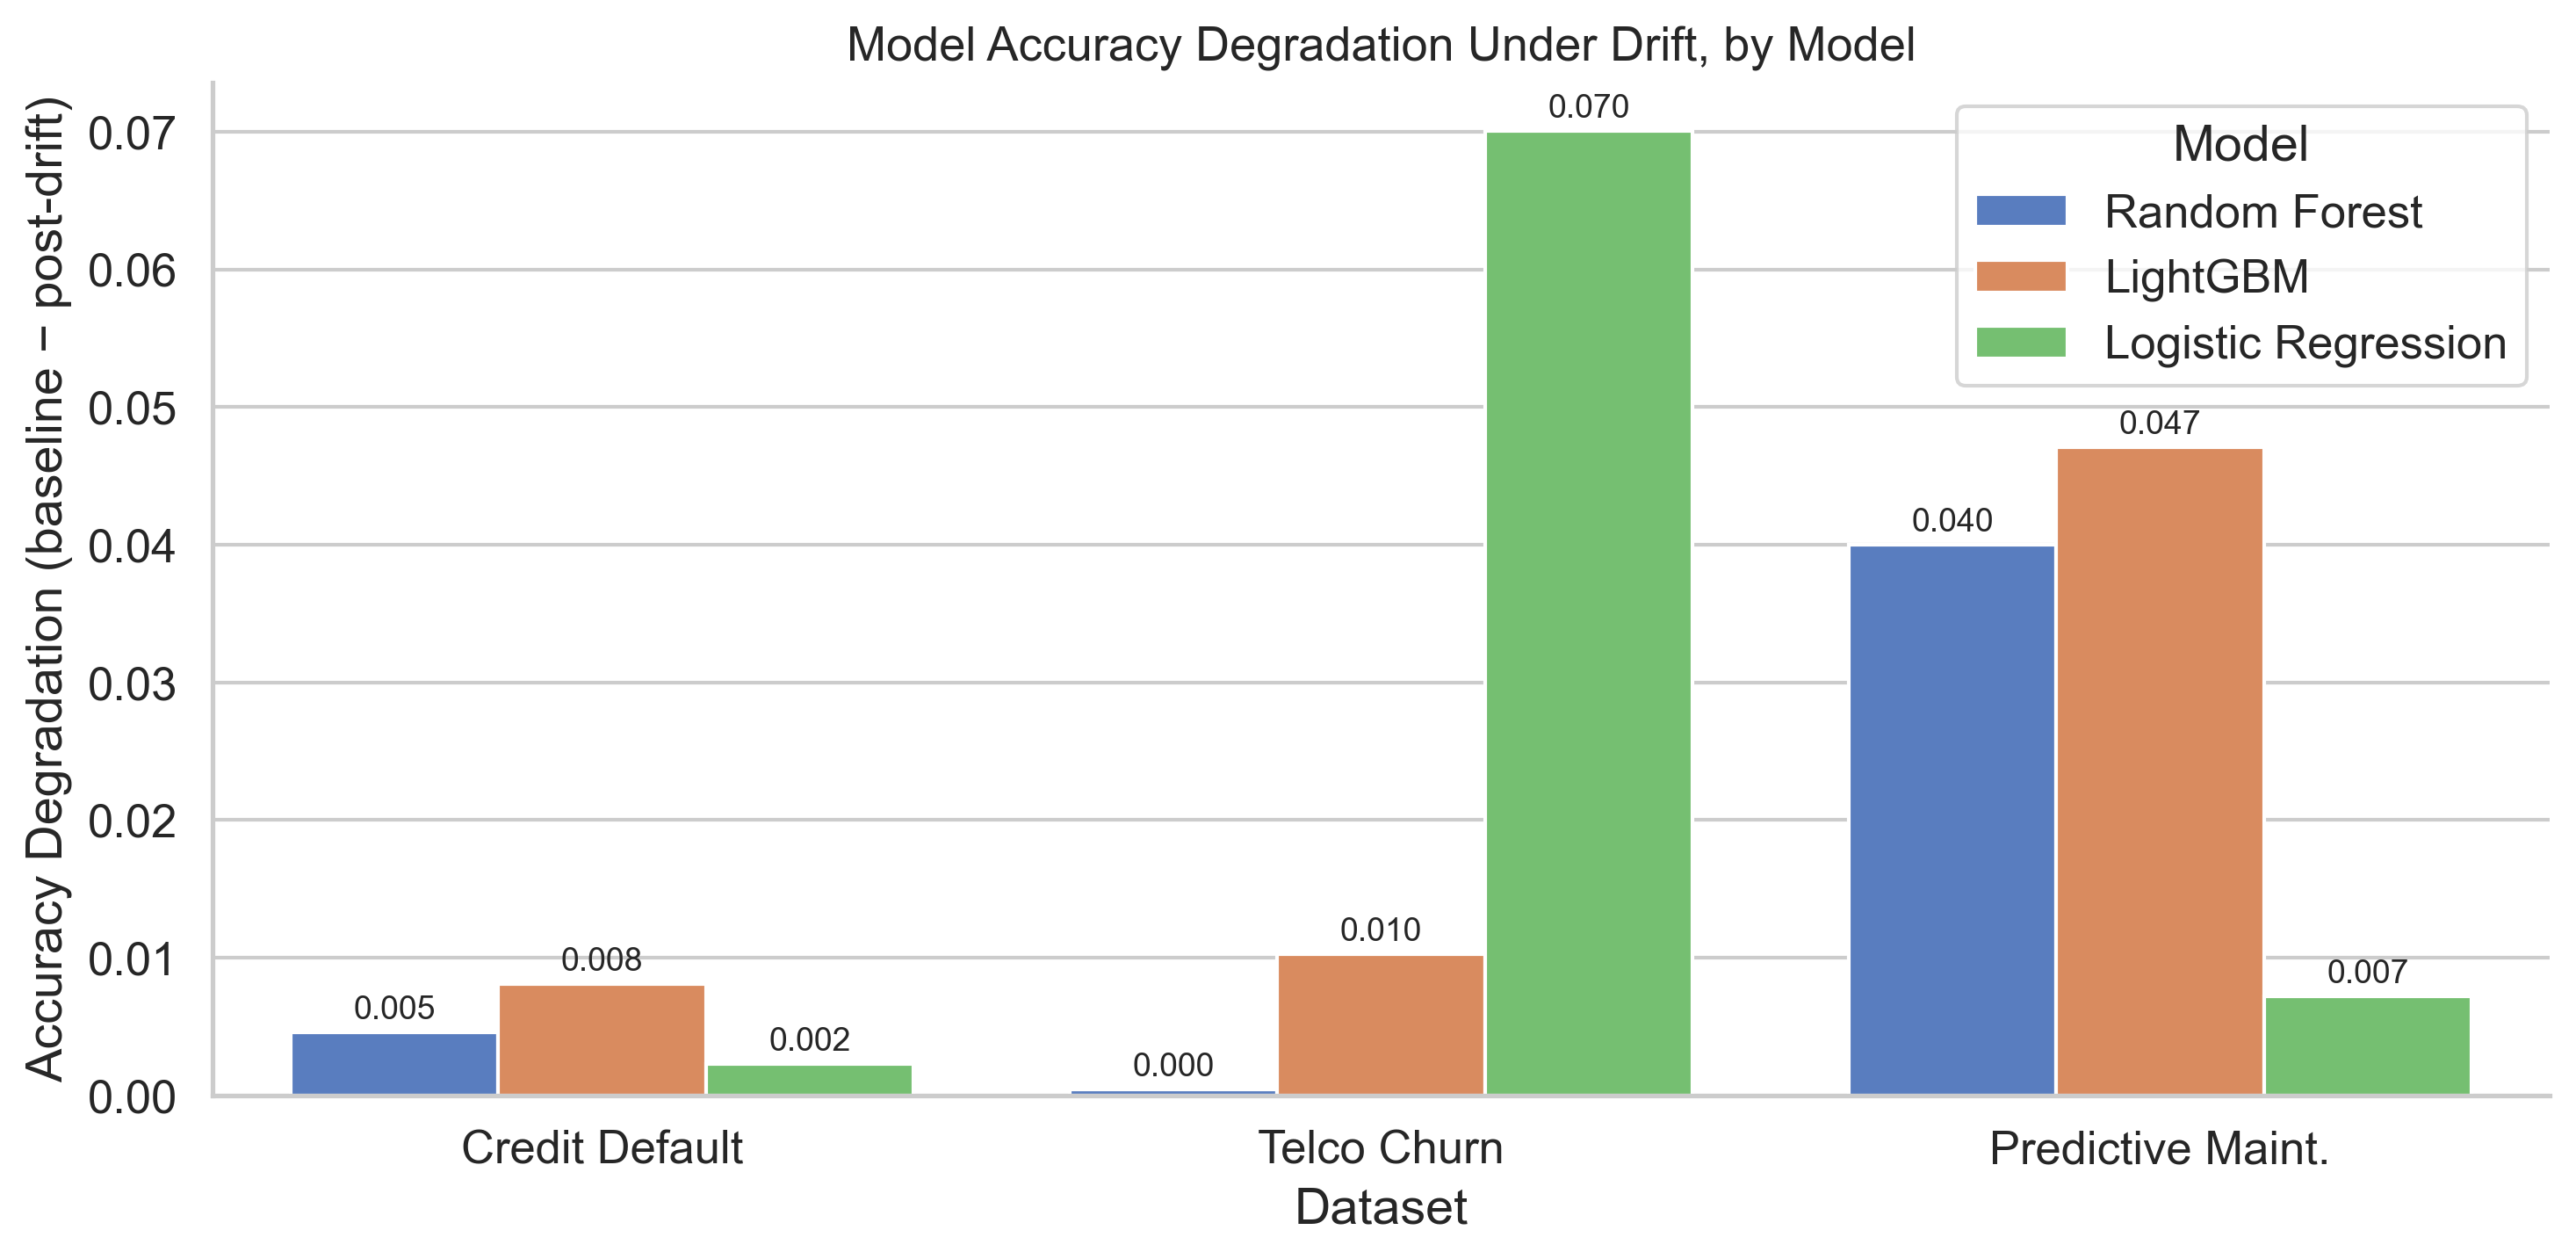
\includegraphics[width=\columnwidth]{../../04_results/plots/fig8_model_robustness.png}
\caption{Mean accuracy degradation (baseline minus post-drift accuracy) by model, per dataset. Random Forest's advantage over LightGBM holds in direction across all three datasets. Logistic Regression's poor aggregate performance is driven almost entirely by Telco Churn, where it is the least robust model by a wide margin; on the other two datasets it is competitive with or better than both ensembles.}
\label{fig:modelrobustness}
\end{figure}

\section{Discussion}

\subsection{The Priority Hierarchy}

Integrating the findings across all four research questions yields a priority hierarchy for resource-constrained drift monitoring deployment:

\textbf{First priority: monitoring regime configuration.} The constraint analysis demonstrates that monitoring frequency and detection window size collectively produce the largest performance variation in the study, a 37-fold range in detection delay, with effect sizes ($\rho \approx 0.49$--$0.54$) substantially larger than those for detector choice ($r \approx 0.15$). System designers should set monitoring frequency as high as their compute budget allows and choose the smallest detection window that provides acceptable statistical power for their expected drift magnitude.

\textbf{Second priority: drift type awareness.} Gradual drift is systematically and substantially harder to detect than sudden or recurring drift ($r \approx 0.30$, medium effect). A system calibrated and validated exclusively on sudden-change scenarios, as most benchmark studies are, may provide misleading performance guarantees for gradual drift, which is arguably more common in real deployment environments where populations shift slowly. Practitioners should explicitly test their monitoring configurations against gradual drift scenarios and consider lower detection thresholds or smaller window sizes if gradual drift is expected.

\textbf{Third priority: algorithm and model selection.} After the monitoring regime and drift type considerations are addressed, detector choice and model choice represent relatively smaller sources of performance variation. Wasserstein distance offers the best detection capability at moderate computational cost; KS offers strong detection at higher compute; PSI offers acceptable detection at lowest compute. Random Forest is the recommended base model in non-stationary environments where retraining is costly.

\subsection{The Reference Window Threshold}

The threshold finding for reference window size, that 500 samples is functionally equivalent to an unlimited reference window, has a direct practical implication for memory-constrained deployment. A monitoring system that stores and maintains 500 reference samples per feature achieves full detection quality without requiring access to the entire historical training dataset. This supports the design of streaming monitoring pipelines in which reference data can be pruned periodically without sacrificing detection performance.

\subsection{Positioning Relative to Prior Work}

This study's findings complement and extend the large-scale benchmark of Barros \& Santos~\cite{barros2018} in two directions. First, while Barros \& Santos~\cite{barros2018} find that no single detector dominates across all conditions, this study reveals that the between-detector differences are secondary to the effect of monitoring configuration, a finding that reframes the focus from algorithm selection to system design. Second, the gradual drift finding of this study, obtained for distribution-based label-free detectors, replicates the qualitative finding of Barros \& Santos~\cite{barros2018} for supervised error rate-based detectors, suggesting that gradual drift resistance is a detection-paradigm-level challenge rather than an algorithm-specific limitation.

The model robustness finding, that Random Forest outperforms LightGBM under drift, appears to contrast with the finding of Pathi~\cite{pathi2025} that gradient boosting achieves the best accuracy-stability balance in some datasets. The discrepancy is attributable to the difference in evaluation task: Pathi~\cite{pathi2025} measures PSI as a static population stability index, while this study measures dynamic accuracy degradation under experimentally injected drift. The two metrics capture different aspects of model stability, and both contribute to a complete picture.

\subsection{Limitations}

This study focuses exclusively on tabular binary-classification tasks; the findings may not generalise to image, text, or multi-class problems. Drift is simulated via controlled statistical transformations rather than observed as a naturally occurring process; real-world drift may involve correlated multi-feature shifts that are qualitatively different. All three detectors are applied feature-wise (univariate), potentially missing multivariate distributional changes involving feature correlation structure. Monitoring configurations are evaluated across three constraint levels per parameter; finer resolution within the parameter space may reveal more detailed tradeoff structure.

\section{Conclusion}

This paper presents the first systematic constraint-aware evaluation of three lightweight distribution-based drift detectors across 8,100 experimental configurations. The central finding is that the configuration of the monitoring system, specifically monitoring frequency and detection window size, produces a 37-fold range in detection delay, substantially exceeding the between-detector performance gap. This result establishes that the choice of \emph{how} a monitoring system is configured is more consequential than the choice of \emph{which} algorithm it uses.

Gradual drift is systematically and substantially harder to detect than sudden or recurring drift across all detectors and constraint configurations, with a medium effect size ($r \approx 0.30$) that significantly exceeds the detector-comparison effects. The equivalence of sudden and recurring drift detection performance indicates that distribution-based detectors respond to concept recurrence with the same sensitivity as to novel sudden shifts.

A reference window threshold of approximately 500 samples provides detection performance equivalent to an unlimited reference, supporting memory-efficient monitoring pipeline design. Random Forest shows the greatest robustness to drift-induced performance degradation among the three evaluated model architectures.

The practical guidance distilled from these findings is a ranked priority hierarchy: configure the monitoring regime first, account for drift type second, and select the detector and model third. Deployment decisions should be informed by constraint-aware evaluation rather than benchmark results obtained under idealised conditions that do not represent the resource environments of real production systems.

\bibliographystyle{IEEEtran}
\bibliography{references}

\end{document}
